\documentclass[UTF8,a4paper,12pt]{ctexbook} 

\usepackage{graphicx}%学习插入图
\usepackage{verbatim}%学习注释多行
\usepackage{booktabs}%表格
\usepackage{geometry}%图片
\usepackage{amsmath}
\usepackage{amssymb}
\usepackage{listings}%代码
\usepackage{xcolor}  %颜色
\usepackage{enumitem}%列表格式
\setenumerate[1]{itemsep=0pt,partopsep=0pt,parsep=\parskip,topsep=5pt}
\setitemize[1]{itemsep=0pt,partopsep=0pt,parsep=\parskip,topsep=5pt}
\setdescription{itemsep=0pt,partopsep=0pt,parsep=\parskip,topsep=5pt}
\usepackage{tcolorbox}
\usepackage{algorithm}  %format of the algorithm
\usepackage{algorithmic}%format of the algorithm
\usepackage{multirow}   %multirow for format of table
\usepackage{tabularx} 	%表格排版格式控制
\usepackage{array}	%表格排版格式控制
\usepackage{hyperref} %超链接 \url{URL}
\usepackage{tikz}
\usepackage{dirtree}


\usetikzlibrary{intersections,
	positioning,
	petri,
	backgrounds,
	fit,
	decorations.pathmorphing,
	arrows,
	arrows.meta,
	bending,
	calc,
	intersections,
	through,
	backgrounds,
	shapes.geometric,
	quotes,
	matrix,
	trees,
	shapes.symbols,
	graphs,
	math,
	patterns,
	external}

\setmainfont{Times New Roman}
\graphicspath{{figure/}}
\CTEXsetup[format+={\flushleft}]{section}
%%%% 段落首行缩进两个字 %%%%
\makeatletter
\let\@afterindentfalse\@afterindenttrue
\@afterindenttrue
\makeatother
\setlength{\parindent}{2em}  %中文缩进两个汉字位

%%%% 下面的命令重定义页面边距,使其符合中文刊物习惯 %%%%
\addtolength{\topmargin}{-54pt}
\setlength{\oddsidemargin}{0.63cm}  % 3.17cm - 1 inch
\setlength{\evensidemargin}{\oddsidemargin}
\setlength{\textwidth}{14.66cm}
\setlength{\textheight}{24.00cm}    % 24.62

%%%% 下面的命令设置行间距与段落间距 %%%%
\linespread{1.4}
\setlength{\parskip}{0.5\baselineskip}
\geometry{left=1.6cm,right=1.8cm,top=2cm,bottom=1.7cm} %设置文章宽度
\pagestyle{plain} 		  %设置页面布局

%代码效果定义
\definecolor{mygreen}{rgb}{0,0.6,0}
\definecolor{mygray}{rgb}{0.5,0.5,0.5}
\definecolor{mymauve}{rgb}{0.58,0,0.82}
\lstset{ %
	backgroundcolor=\color{white},   % choose the background color
	basicstyle=\footnotesize\ttfamily,      % size of fonts used for the code
	%stringstyle=\color{codepurple},
	%basicstyle=\footnotesize,
	%breakatwhitespace=false,         
	%breaklines=true,                 
	%captionpos=b,                    
	%keepspaces=true,                 
	%numbers=left,                    
	%numbersep=5pt,                  
	%showspaces=false,                
	%showstringspaces=false,
	%showtabs=false,        
	columns=fullflexible,
	breaklines=true,                 % automatic line breaking only at whitespace
	captionpos=b,                    % sets the caption-position to bottom
	tabsize=4,
	commentstyle=\color{mygreen},    % comment style
	escapeinside={\%*}{*)},          % if you want to add LaTeX within your code
	keywordstyle=\color{blue},       % keyword style
	stringstyle=\color{mymauve}\ttfamily,     % string literal style
	frame=single,
	rulesepcolor=\color{red!20!green!20!blue!20},
	% identifierstyle=\color{red},
	language=c++,
}
 \author{\kaishu 郑华}
 \title{Linux 系统编程 笔记}
 
\begin{document}          %正文排版开始
 	\maketitle
 
\chapter{基础查漏补缺}
	\section{系统编程简介}
		用程序完成Linux 命令等干的事情。
	
	\section{进程组、会话}
		参考:\url{https://www.cnblogs.com/zengyiwen/p/5755191.html}
		
		\textbf{进程组}是一组相关进程的集合,\textbf{会话}是一组相关进程组的集合。
	
		
		\paragraph{进程ID 组成}这样说来,一个进程会有如下\verb|ID| :
			\begin{itemize}
				\item \verb|PID |:进程的唯一标识。对于多线程的进程而言,所有线程调用getpid函数会返回相同的值。
				\item \verb|PGID |:进程组ID。每个进程都会有进程组ID,表示该进程所属的进程组。默认情况下新创建的进程会继承父进程的进程组ID。
				\item \verb|SID |:会话ID。每个进程也都有会话ID。默认情况下,新创建的进程会继承父进程的会话ID。
			\end{itemize}
		
			\subparagraph{查看ID}\verb|->|
			
			可以调用如下\verb|命令|来查看所有进程的层次关系:
			\verb|ps -ejH |或
			\verb|ps axjf |
			
			可以调用以下\textbf{函数}获取进程组ID跟会话ID.
			\verb|pid_t getpgrp(void);| 或
			\verb|pid_t getsid(pid_t pid); |
			
		
			新进程\textbf{默认继承}父进程的\textit{进程组ID和会话ID},如果都是默认情况的话,那么追根溯源可知,所有的进程应该有共同的进程组ID和会话ID。
			实际情况并非如此,系统中存在很多不同的会话,每个会话下也有不同的进程组。
			为何会如此呢?
			
			就像家族企业一样,如果从创业之初,所有家族成员都墨守成规,循规蹈矩,默认情况下,就只会有一个公司、一个部门。但是也有些“叛逆”的子弟,愿意为家族公司开疆拓土,愿意成立新的部门。这些新的部门就是新创建的进程组。如果有子弟“离经叛道”,甚至不愿意呆在家族公司里,他别开天地,另创了一个公司,那这个新公司就是新创建的会话组。由此可见,系统必须要有改变和设置进程组ID和会话ID的函数接口,否则,系统中只会存在一个会话、一个进程组。
		
		\paragraph{进程组、会话}
			进程组和会话是为了支持shell作业控制而引入的概念。
			当有新的用户登录Linux时,登录进程会为这个用户创建一个会话。用户的登录shell就是会话的首进程。会话的首进程ID会作为整个会话的ID。会话是一个或多个进程组的集合,囊括了登录用户的所有活动。
				\begin{figure}[H]
					\centering
					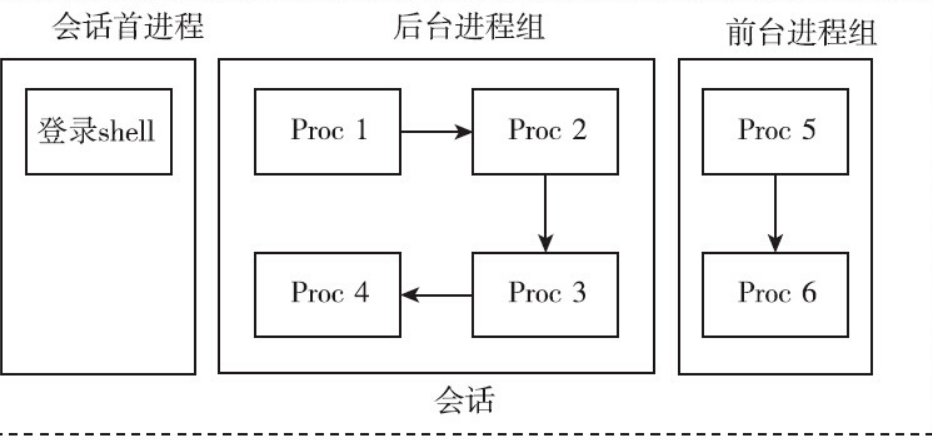
\includegraphics[scale=0.5]{huihua.png}
					\caption{会话结构}
				\end{figure}
			
			在登录shell时,用户可能会使用管道,让多个进程互相配合完成一项工作,这一组进程属于同一个进程组。
			
			最常见的创建进程组的场景就是在shell中执行管道命令,代码如下:\verb|cmd1 | cmd2 | cmd3|
			
			下面用一个最简单的命令来说明,其进程之间的关系如图\ref{processG}所示。
			\verb|ps ax|grep nfsd|
				
					\begin{figure}[H]
						\centering
						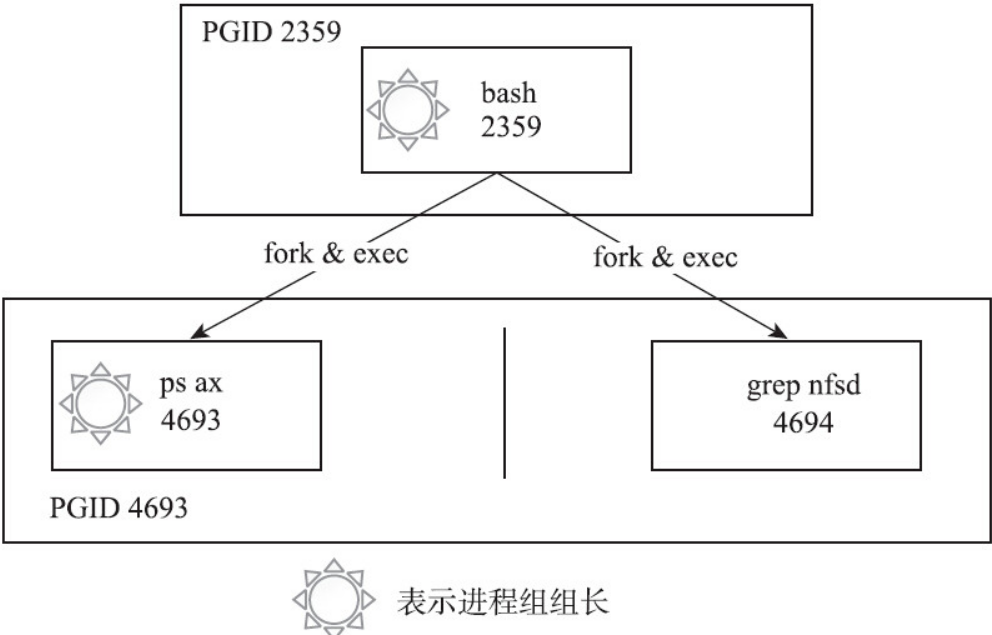
\includegraphics[scale=0.5]{processGroup.png}
						\caption{进程组结构演示}
						\label{processG}
					\end{figure}
			 
			 ps进程和grep进程都是bash创建的子进程,两者通过管道协同完成一项工作,它们隶属于同一个进程组,其中ps进程是进程组的组长。
			 
			 进程组的概念并不难理解,可以将人与人之间的关系做类比。一起工作的同事,自然比毫不相干的路人更加亲近。shell中协同工作的进程属于同一个进程组,就如同协同工作的人属于同一个部门一样。
			 
			 引入了进程组的概念,可以更方便地管理这一组进程了。比如这项工作放弃了,不必向每个进程一一发送信号,可以直接将信号发送给进程组,进程组内的所有进程都会收到该信号。
			 
	\section{errno 与 perror()}
		使用perror 函数打印对应errno对应的错误信息。
	
		\begin{lstlisting}
	int fd = open("english",O_RDWR);
	if(fd == -1)
	{
		perror("Message");
	}
	
	//--> Message: 错误信息
		\end{lstlisting}
		
		\paragraph{char* strerror(int errno)}打印对应的错误信息。
	
	\section{逻辑地址与物理地址}
		从逻辑地址到物理地址的映射称为地址重定向。分为:
				
		静态重定向--在程序装入主存时已经完成了逻辑地址到物理地址和变换,在程序执行期间不会再发生改变。
				
		动态重定向--程序执行期间完成,其实现依赖于硬件地址变换机构,如基址寄存器。
				
		\textbf{逻辑地址}:CPU所生成的地址。CPU产生的逻辑地址被分为 :p (页号) 它包含每个页在物理内存中的基址,用来作为页表的索引;d (页偏移),同基址相结合,用来确定送入内存设备的物理内存地址。
				
		\textbf{物理地址}:内存单元所看到的地址。
		
		用户程序看不见真正的物理地址。用户只生成逻辑地址,且认为进程的地址空间为0到max。物理地址范围从R+0到R+max,R为基地址,地址映射-将程序地址空间中使用的逻辑地址变换成内存中的物理地址的过程。由内存管理单元(MMU)来完成。
		
	\section{UID、 EUID}
	
	
\chapter{虚拟地址空间}
	\dirtree{%
			.1  虚拟地址内存.
			.2  内核区.
			.3  内存管理.
			.3  进程管理.
			.3  虚拟文件管理.
			.3  设备管理.
			.2  环境变量 env.
			.2  命令行参数 *argv[].
			.2  栈空间.
			.2  共享库的存储器映射区.
			.2  堆空间.
			.2  全局变量共享区.
			.3  bss 未初始化全局.
			.3  data 初始化全局.
			.2  text.
		}
		
	\begin{figure}[H]
		\centering
		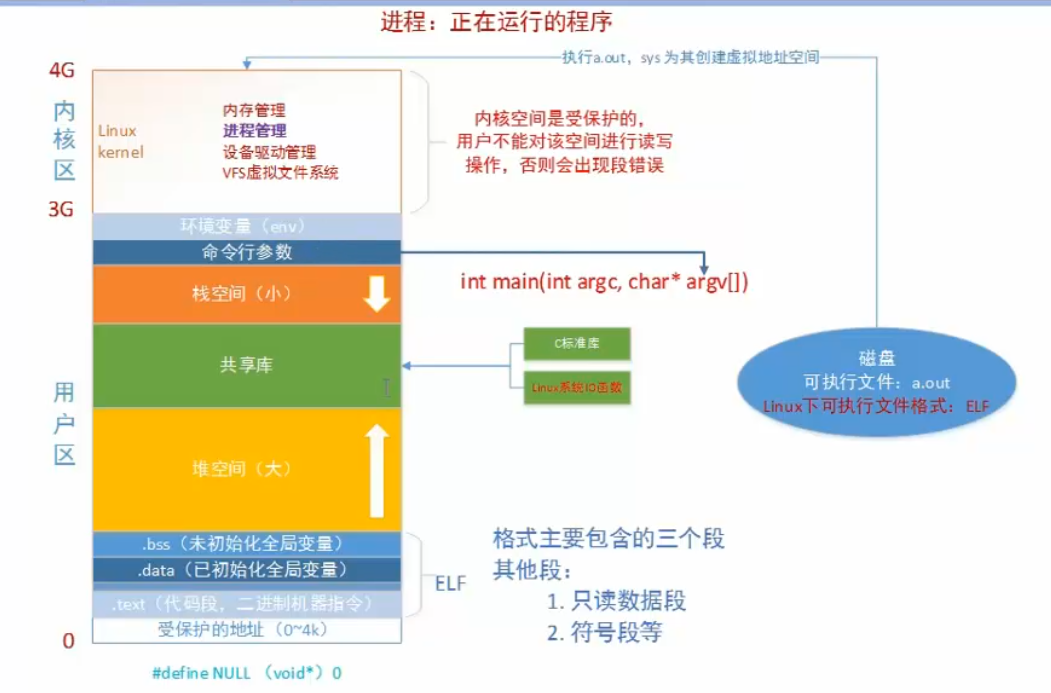
\includegraphics[scale=0.5]{memoryMap.png}
		\caption{内存地址空间}
	\end{figure}
	

\chapter{文件操作}
	\dirtree{%
		.1  读写操作.
		.2  读取.
		.3  Open.
		.3  ReadWrite.
		.3  Lseek.
		.2  文件状态.
		.3  Stat.
		.3  属性.
		.2  内容复制.
		.3  dup.
		.3  dup2.
	}
	
		\begin{figure}[htb]
			\centering
			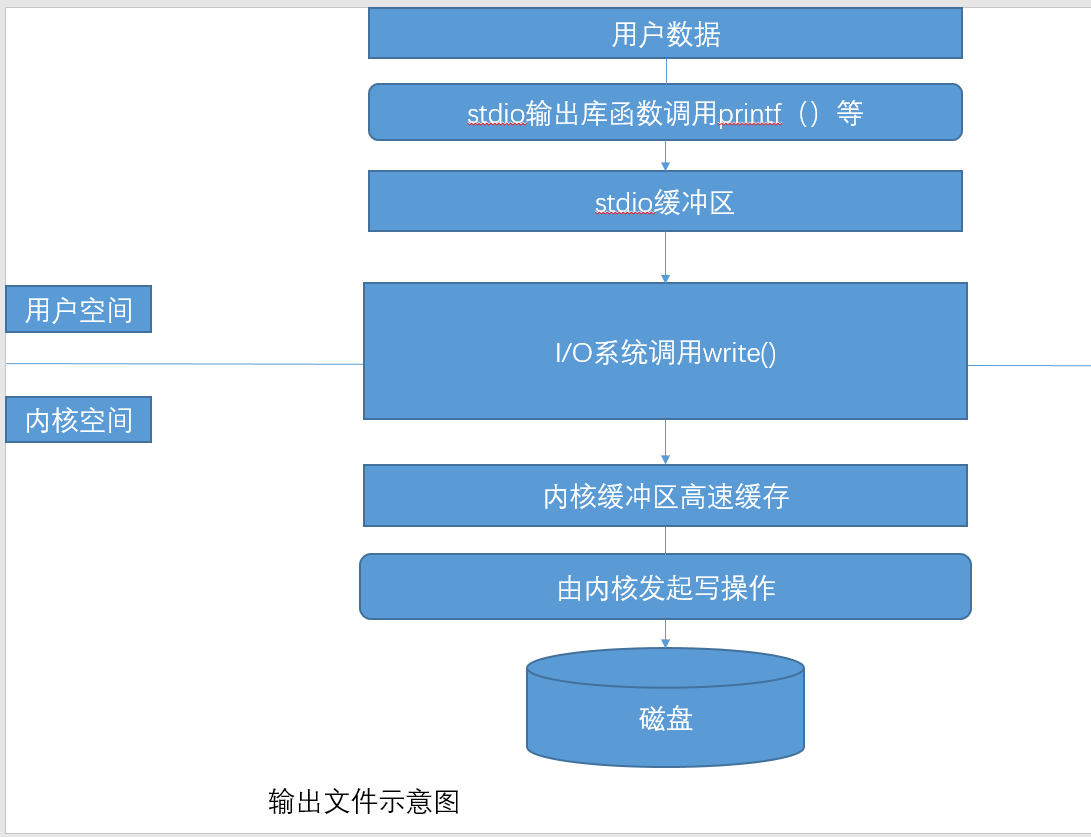
\includegraphics[scale=0.35]{io.png}
			\caption{I/O 系统结构}
		\end{figure}
			
	\section{文件描述符表}
		每打开一个文件就占用一个文件描述符,系统通过文件描述符找到对应的磁盘进行文件操作。
		
		并且文件描述符的分配遵循:在空闲的文件描述符集合中,选取最小的分配给当前文件
	
		系统占用前三个描述符, 并默认打开,分别为stdin(0):\verb|STDIN_FILENO|,stdout(1)\verb|STDOUT_FILENO|,stderr(2)\verb|STDERR_FILENO|
	
	\section{阻塞非阻塞}
		阻塞:到达该函数后,必须执行完才能继续向下执行
		
		非阻塞:到达后,基础处理后面代码,等待消息再处理。
		
		\verb|/dev/tty |类似与c++ 中的this, 指向当前终端。
		
		\subparagraph{要点}
			\begin{itemize}[itemindent = 1em]
				\item 属于\textbf{文件的属性}
				\item 普通文件\textbf{默认不阻塞}
				\item 终端设备\verb|/dev/tty 或 STDOUT_FILENO 或 管道 或 套接字|等\textbf{默认阻塞}
			\end{itemize}
		
	\section{读写操作}		
		\paragraph{open()}打开文件(文件路径,读写选项,默认权限)
			\subparagraph{函数原型}\fbox{int open(const char* path, int flags, mode\_t mode)}
				
			\subparagraph{参数说明}
				\begin{itemize}[itemindent = 1em]
					\item \verb|返回 |文件描述符
					\item \verb|path |文件路径
					\item \verb|flag |文件打开方式,读、写、追加、创建等
					\item \verb|mode |针对当flags 中具有创建文件权限时,指定文件权限的参数
				\end{itemize}
				
			\subparagraph{示例}
				\verb|->|
				\begin{lstlisting}[frame = L, xleftmargin = .1\textwidth]
	int fd = open("startUp",O_RDONLY);
	if(fd == -1)
		errExit("open");
		
	fd = open("w.log",O_WRONLY | O_CREAT | O_TRUNC | O_APPEN, S_IRUSR | S_IWUSER);
				\end{lstlisting}
	
		\paragraph{close()}
			\subparagraph{函数原型}\fbox{int close(int fd)}
				
			\subparagraph{参数说明}fd 文件描述符		
			
		\paragraph{lseek()}修改文件的偏移量,文件偏移量是指执行下一个read()或write() 操作的文件起始位置。
			\subparagraph{函数原型}\fbox{off\_t lseek(int fd, off\_t offset, int whence)}
				
			\subparagraph{参数说明}
				\begin{itemize}[itemindent = 1em]
					\item \verb|offset |指定一个以字节为单位的数值,定义偏移量。
					\item \verb|whence |表明参照哪个基点来解释offset 参数\verb|[SEEK_SET, SEEK_END)|,
						\begin{description}[itemindent = 1em]
							\item{\verb|SEEK_SET|}文件开始位置
							\item{\verb|SEEK_CUR|}当前位置
							\item{\verb|SEEK_END|}文件结束位置的后一个位置
						\end{description}
				\end{itemize}		
		\paragraph{read()}将文件内容读至缓存
			\subparagraph{函数原型}\fbox{ssize\_t read(int fd, void *buffer, size\_t count)}
				
			\subparagraph{参数说明}
				\begin{itemize}[itemindent = 1em]
					\item \verb|返回值 |返回实际读取的字节数,如果遇到EOF 返回0,出现错误返回-1.
					\item \verb|buffer |用来存放输入数据的内存地址
					\item \verb|count |指定最多能读取的字节数
				\end{itemize}	
					
		\paragraph{readv()}
			\subparagraph{函数原型}
				
			\subparagraph{参数说明}	
				
		\paragraph{write()}将缓冲数据写入文件
			\subparagraph{函数原型}\fbox{ssize\_t write(int fd, void* buffer, size\_t  count)}
				
			\subparagraph{参数说明}
				\begin{itemize}[itemindent = 1em]
					\item \verb|返回值 |返回实际写入文件的字节数
					\item \verb|buffer |数据内存地址
					\item \verb|count |预从buffer 写入文件的数据字节数
				\end{itemize}
		
		\paragraph{writev()}将缓冲区数据写入文件
			\subparagraph{函数原型}
				
			\subparagraph{参数说明}		
		\paragraph{truncate()}
			\subparagraph{函数原型}
				
			\subparagraph{参数说明}		
		\paragraph{ftruncate()}
			\subparagraph{函数原型}
				
			\subparagraph{参数说明}		
		\paragraph{ioctl()}
			\subparagraph{函数原型}
				
			\subparagraph{参数说明}
					
	\section{文件属性}
		\subsection{属性操作}
			\begin{figure}[H]
				\centering
				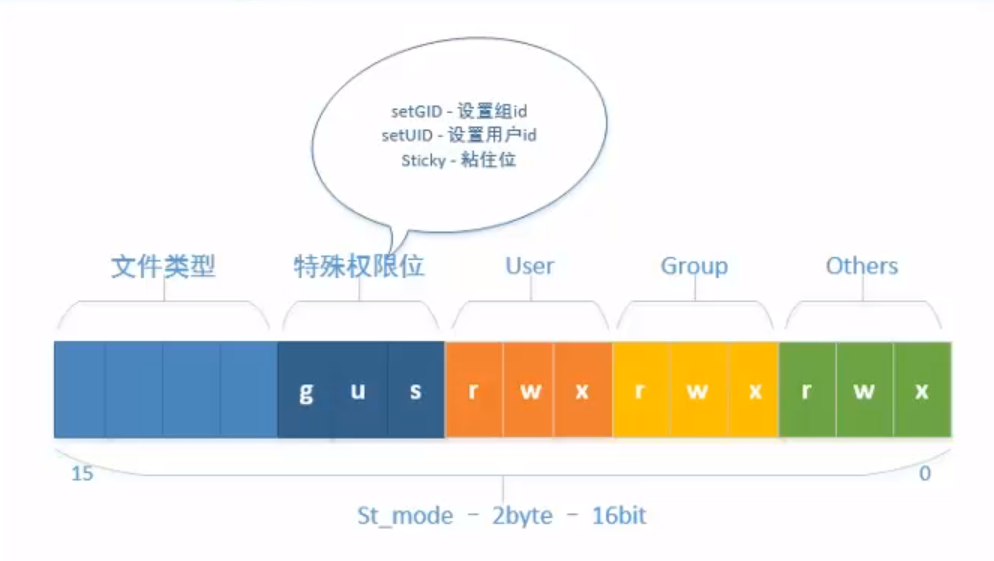
\includegraphics[scale=0.5]{fileStat_mode.png}
				\caption{文件属性表示图}
				\label{st_mode}
			\end{figure}
		
		文件类型包括如下7种:
		\begin{itemize}[itemindent = 1em]
			\item \verb|S_IFSOCK | 套接字
			\item \verb|S_IFLNK | 符号链接(软链接)
			\item \verb|S_IFREG | 普通文件
			\item \verb|S_IFBLK | 块设备
			\item \verb|S_IFDIR | 目录
			\item \verb|S_IFCHR | 字符设备
			\item \verb|S_IFIFO | 管道
			\item \verb|*S_IFMT | 类型掩码
		\end{itemize}
			
		\paragraph{stat()}查看文件大小、时间戳、权限权限等基本属性,类似\verb|ls -l fileName|
			\subparagraph{函数原型}\fbox{int stat(const char* path, struct stat* buf)}
					
			\subparagraph{参数说明}
				输入输出参数:\verb|struct stat* |,主要包括
				\begin{itemize}[itemindent = 1em]
					\item 文件的设备编号
					\item i节点
					\item 文件的类型和存取权限
					\item 用户ID
					\item 组ID
					\item 文件大小
					\item 硬链接计数
					\item 修改时间等
				\end{itemize}
			
			\subparagraph{判断文件的类型示例}st 为struct stat结构体,st\_mode 表示其中文件的类型和存取权限,如图\ref{st_mode}所示。
				\verb|if(st.st_mode & S_IFMT == S_IFREG)|
			
		\paragraph{lstat()}
			\subparagraph{函数原型}\fbox{int lstat(const char* path, struct stat* buf)}
			
			\subparagraph{与stat的区别}读取软链接文件的方式不同。
				\begin{itemize}[itemindent = 1em]
					\item \verb|stat() | 函数会对软链接文件进行解析,读取的是软链接指向的文件
					\item \verb|lstat() | 则只是对传进去的文件进行分析,如果是软链接则不继续解析、追踪。
				\end{itemize}
				
		\paragraph{fstat()}操作同stat(),区别是第一个参数不同
			\subparagraph{函数原型}\fbox{int fstat(int fd, struct stat* buf)}	
			
	\subsection{权限操作}	
		\paragraph{access()} 测试当前用户指定的文件是否具有某种属性。
		
		\paragraph{chmod()}
		
		\paragraph{chown()}
		
		\paragraph{trucncate()}修改文件大小,传进去的大小比原来小,删掉后面的内容,比原来大,则向后拓展。
			\subparagraph{函数原型}\fbox{int truncate(const char *path, off\_t length)}
			
		\paragraph{ftruncate()}同truncate.
			\subparagraph{函数原型}\fbox{int ftruncate(int fd, off\_t length)}
		
	\subsection{目录操作}
		\paragraph{rename()}
		
		\paragraph{chdir()} 修改当前进程的路径,cd
		
		\paragraph{getcwd()} 获取当前工作目录路径,pwd
		
		\paragraph{mkdir()} 创建目录
		
		\paragraph{rmdir()} 删除目录
		
		\paragraph{opendir()} 打开一个目录,遍历
		
		\paragraph{readdir()} 
		
		\paragraph{closedir()}
	
		
	\section{文件重定向}		
		\paragraph{dup()}复制文件描述符
			\subparagraph{函数原型}\fbox{int dup(int oldFd)}
				
			\subparagraph{参数说明}
				\begin{itemize}[itemindent = 1em]
					\item \verb|oldFd |要复制的文件描述符
					\item \verb|返回值 |返回新的文件描述符,同文件描述符分配过程,取最小的
					\item \verb|dup 调用成功 |则两个文件描述符指向同一个文件(oldFd)
				\end{itemize}	
				
		\paragraph{dup2()}复制文件描述符
			\subparagraph{函数原型}\fbox{int dup2(int oldFd, int newFd)}
				
			\subparagraph{参数说明}
				\begin{itemize}[itemindent = 1em]
					\item oldFd = dup 中的oldFd
					\item newFd = dup 中的返回值
					\item \verb|dup2 调用成功 |则两个文件描述符都指向同一个文件(oldFd)
				\end{itemize}		
	
		\paragraph{fcntl()}变更文件属性
			\subparagraph{函数原型}\fbox{int fcntl(int fd, int cmd, ...)}
			
			\subparagraph{参数说明}
				变参主要针对不同的cmd,体现出不同,cmd 具有如下几种: 
				\begin{itemize}[itemindent = 1em]
					\item \verb|F_DUPFD |复制一个已有文件描述符,同dup				
					\item \verb|F_GETFL |获取文件状态标识\verb|int flag = fcntl(fd, F_GETFL);|
					\item \verb|F_SETFL |设置文件状态\verb|fcntl(fd, F_SETFL, flag);|,文件已经打开,然后需要修改文件属性。
				\end{itemize}
	
\chapter{线程}
	\section{线程创建}
		\paragraph{pthread\_create()}
				\subparagraph{函数原型}\fbox{pthread\_create(pthread\_t*  id, pthread\_attr\_t* attr, void*(*start\_routine)(void*), void* arg)}
					
				\subparagraph{参数说明}
					\begin{itemize}[itemindent = 1em]
						\item \verb|void* (*start_routine) (void*)|:这里是个陷阱,如果使用成员函数会存在一个参数不匹配问题,因为成员函数有一个隐含的第一参数this,而this 为类指针类型,与void* 不匹配,造成了notMatch 错误。
						\item \verb|*id |输出参数
						\item \verb|*attr |用于设置父子线程分离,完成自我回收
					\end{itemize}
				
				\subparagraph{创建时设置属性分离}使得子线程完成自我回收。
					\begin{itemize}[itemindent = 1em]
						\item 线程属性类型\verb|othread_attr_t attr;|
						\item 对线程属性变量初始化\fbox{ptread\_attr\_init(pthread\_attr\_t* attr)}
						\item 设置线程分离属性\fbox{pthread\_attr\_setdetachstate(pthread\_attr\_t* attr, int detachstate)}
							\begin{itemize}[itemindent = 1em]
								\item \verb|attr |线程属性
								\item \verb|detachstate | 分离类型:\verb|PTHREAD\_CREATE\_DETACH| 非分离类型:\verb|..CREATE\_JOINABLE|
							\end{itemize}
						\item 释放线程资源函数\fbox{pthread\_attr\_destroy(pthread\_attr\_t *attr)}
					\end{itemize}
		\paragraph{创建线程后与原进程的关系}\verb|->|
			\begin{itemize}[itemindent = 1em]
				\item 创建线程后,地址空间没有变化
				\item \textbf{进程退化成了线程}-主线程
				\item 创建出的子线程和主线程 \textbf{共用地址空间}
				\item \textit{主线程和子线程} \textbf{在内核区有了各自的PCB},而子线程的PCB是从主线程拷贝过来的,\textbf{OS进程调度的时候是根据PCB进行的}
			\end{itemize}	
			
			\subparagraph{共享、私有内容}\textit{除了栈区都共享},因此\textbf{线程间通信}可以\textbf{使用其他区域的任何变量}来实现。
				\textbf{有几个线程,栈会平均分为几份}。
				
		\paragraph{进程ID、线程号、线程ID}\verb|->|
			\begin{itemize}[itemindent = 1em]
				\item \textbf{进程ID} \verb|PID|- 给用户看的
				\item \textbf{线程号} \verb|LWP|- 给内核看的\verb|ps -Lf _PID|,一般情况PID相同,LWP不同
				\item \textbf{线程ID} \verb|TID|- 给用户看的
			\end{itemize}
		
		\paragraph{pthread\_self()} 查看当前线程的线程id。
	
	\section{线程运行}
		\paragraph{pthread\_detach()}线程分离,调用该函数后,主线程不需要调用\verb|othread\_join()|完成pcb 的回收,子线程负责自我回收。
			\subparagraph{函数原型}\fbox{int pthread\_detach(pthread\_t thread)}
	
	\section{线程终止}	
		\paragraph{pthread\_exit()}单个线程退出,对子线程无影响,但是PCB没有回收
			\subparagraph{函数原型}\fbox{void pthread\_exit(void *retval)} 输出参数:退出信息,此参数必须是全局的
		
		\paragraph{pthread\_join()}主线程阻塞等待给定子线程结束,并回收资源(PCB)
			\subparagraph{函数原型}\fbox{void pthread\_join(pthread\_t thread, void **retval)} 输出内存:退出信息。
		
	
	\section{线程同步}
		\paragraph{pthread\_mutex\_init()}
		\paragraph{pthread\_mutex\_destroy()}
		\paragraph{pthread\_mutex\_lock()} 如果没有上锁,上锁; 如果已经上锁了,阻塞等待,等待锁释放后解除阻塞并上锁。
		\paragraph{pthread\_mutex\_trylock()}非阻塞模式,尝试获取锁并锁住,如果没有上锁,上锁,并返回0;如果锁已经锁住了,返回其他。
		\paragraph{pthread\_mutex\_unlock()}
						 
\chapter{进程}
	\begin{figure}[H]
		\centering
		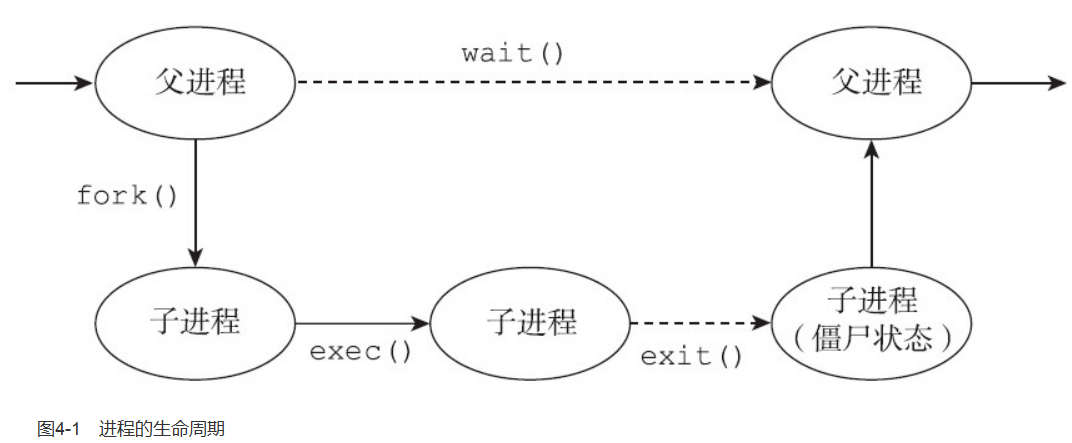
\includegraphics[scale=0.5]{process.png}
		\caption{进程生存演示}
	\end{figure}
	
	\section{进程空间}
		\dirtree{%
			.1 进程空间.
			.2 内核区.
			.3 PCB 进程控制块.
			.2 用户区.
			.3 栈.
			.3 堆.
			.3 bss.
			.3 data.
			.3 text.
			.3 动态库加载区.
			.3 环境变量.
			.3 命令行参数.
		}
	
	\section{进程状态}
		进程的五种状态,如图\ref{proceeStat}所示
			\begin{figure}[H]
				\centering
				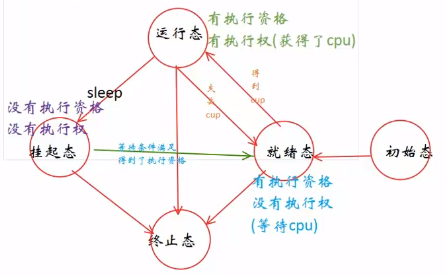
\includegraphics[scale=0.6]{proceeStat.png}
				\caption{进程状态}
				\label{proceeStat}
			\end{figure}
		
	
	\section{PCB 进程控制块}
		位于内核区,名为struct \verb|task_struct|,内容主要包括:
			\begin{itemize}[itemindent = 1em ]
				\item 进程ID \verb|pid_t|,\verb|_t 是| \verb|typedef|使用的简写暗指形式。
				\item 进程状态 \verb|就绪 运行 挂起 终止|
				\item 进程切换时需要保存和恢复的一些CPU寄存器
				\item 描述虚拟地址空间的信息
				\item 描述控制终端信息
				\item 当前工作目录
				\item umask 掩码
				\item 文件描述符表
				\item 信号相关的信息
				\item 用户ID 和组ID
				\item 会话(session)和进程组
				\item 进程可以使用的资源上限(Resource Limit)\verb|ulimit -a|
			\end{itemize}
		
		
	
	\section{进程创建-父子进程}	
		\subsection{fork}
			父子进程执行的操作有一定关系时使用fork 函数完成子进程的创建。
			\paragraph{创建时的动作}\verb|->|
				
				\verb|fork()|会\textbf{产生一个和父进程完全相同的子进程,(进程空间中的\underline{用户区}完全复制,但是内核区部分不同,如PCB中的进程ID,但是文件描述符表相同。)},但子进程在此后多会exec系统调用,出于效率考虑,linux中引入了“写时复制“技术,也就是只有进程空间的各段的内容要发生变化时,才会将父进程的内容复制一份给子进程。在fork之后exec之前两个进程用的是相同的物理空间(内存区),子进程的代码段、数据段、堆栈都是指向父进程的物理空间,也就是说,\textbf{两者的虚拟空间不同,但其对应的物理空间是同一个}。\textbf{当父子进程中有更改相应段的行为发生时,再为子进程相应的段分配物理空间},如果不是因为exec,内核会给子进程的数据段、堆栈段分配相应的物理空间(至此两者有各自的进程空间,互不影响),\textbf{而代码段继续共享父进程的物理空间}(两者的代码完全相同)。而如果是因为exec,由于两者执行的代码不同,子进程的代码段也会分配单独的物理空间。
			
			\paragraph{子进程创建成功后代码的执行位置}\verb|->|
			
				fork 后,分别进入父子进程中的fork 函数,然后执行各自的返回操作,但是用户区的内容是相同的。
				
				也可以这样理解,父进程执行到哪,子进程就执行到哪。
				
				因为栈中保存着函数调用栈,因此函数的调用位置也会存在,而复制的是逻辑空间,因此地址的意义也是一样的。即\textbf{fork时子进程获得父进程数据空间、堆和栈的复制,所以变量的地址、函数的地址(当然是虚拟地址(相对位置))也是一样的}。
			
			
			\paragraph{fork 后父子进程区分}\verb|->|
				\begin{itemize}
					\item 父亲进程\verb|pid > 0|
					\item 孩子进程\verb|pid == 0|
				\end{itemize}
				
			\paragraph{读共享、写复制机制}\verb|->|
	
				\textbf{每个进程都有自己的虚拟地址空间},不同进程的相同的虚拟地址显然可以对应不同的物理地址。因此地址相同(虚拟地址)而值不同没什么奇怪。
				具体过程是这样的:
				
				fork子进程完全复制父进程的栈空间,也复制了页表,但没有复制物理页面,所以这时虚拟地址相同,物理地址也相同,但是会把父子共享的页面标记为“只读”(类似mmap的private的方式),如果父子进程一直对这个页面是同一个页面,知道其中任何一个进程要对共享的页面“写操作”,这时内核会复制一个物理页面给这个进程使用,同时修改页表。而把原来的只读页面标记为“可写”,留给另外一个进程使用。
				
				这就是所谓的“写时复制”。正因为fork采用了这种写时复制的机制,所以fork出来子进程之后,父子进程哪个先调度呢?内核一般会先调度子进程,因为很多情况下子进程是要马上执行exec,会清空栈、堆。。这些和父进程共享的空间,加载新的代码段。。。,这就避免了“写时复制”拷贝共享页面的机会。如果父进程先调度很可能写共享页面,会产生“写时复制”的无用功。所以,一般是子进程先调度滴。
				
				\textbf{假定父进程malloc的指针指向0x12345678, fork 后,子进程中的指针也是指向0x12345678,但是这两个地址都是虚拟内存地址 (virtual memory),经过内存地址转换后所对应的 物理地址是不一样的。所以两个进程中的这两个地址相互之间没有任何关系。}
				
			
				(注1:在理解时,你可以认为fork后,这两个相同的虚拟地址指向的是不同的物理地址,这样方便理解父子进程之间的独立性)
				(注2:但实际上,Linux为了提高 fork 的效率,采用了 copy-on-write 技术,fork后,这两个虚拟地址实际上指向相同的物理地址(内存页),只有任何一个进程试图修改这个虚拟地址里的内容前,两个虚拟地址才会指向不同的物理地址(新的物理地址的内容从原物理地址中复制得到))
				
			
			\paragraph{fork Loop}\verb|->|
			
				当在循环中调用fork时,那么在子进程中也会执行相同的操作。但是不同的是,子进程中的初始变量不同,即循环index 不同。
					\begin{lstlisting}[frame = L, xleftmargin = .1\textwidth]
	for(int i = 0; i < 3; ++i)
	{
		fork();
	}
					\end{lstlisting}
			
				执行上面代码是效果如下:
					\begin{figure}[H]
						\centering
						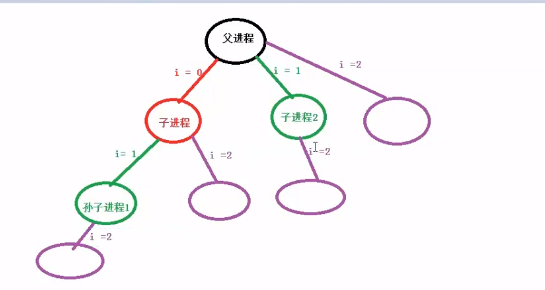
\includegraphics[scale=0.6]{forkLoop.png}
						\caption{forkLoop}
					\end{figure}
					
				过程如下:执行第一次循环时,\verb|i = 0|,产生一个子进程,并且复制父进程的用户区,则此时的子进程的\verb|i = 0|且fork 执行完成,进入\verb|++i |,即子进程产生后的\verb|i = 1|.
				
				在执行第2次fork 时,那么父亲进程与第一次产生的子进程都进入相同的循环\verb|i = 1|,并执行fork,此时则分别产生各自的子进程,并拷贝用户区,此时的\verb|i = 1|,但是fork 执行完进入\verb|++i|, 即相当于父子进程都同时到达\verb|i = 2|.
				
				以此类推,则产生如上图所示效果。	
				
			\paragraph{getpid()、getppid()}\verb|->|
			
				获取当前进程ID:\verb|getpid()|
				
				获取当前进程的父进程ID:\verb|getppid()|	
		
			\paragraph{vfork()}\verb|->|
				
				\subparagraph{相同} vfork() 函数的调用序列和返回值与fork 相同
				
				\subparagraph{不同的是} vfork创建的子进程与父进程共享地址空间,即子进程完全运行在父进程的地址空间上,子进程对虚拟地址空间的修改同样为父进程所见,用vfork创建子进程后,父进程会被阻塞到子进程调用exec或exit。
				
				vfork避免了(fork函数子进程被创建后,仅仅为调用exec执行另一个程序,它对地址空间的复制是多余的)这个问题,减少了不必要的开销。
				
				vfork保证子进程先运行,它调用exec或exit后父进程才能调度运行,fork的父子进程运行顺序不定,取决于内核的调度算法。
				
		\subsection{exec 函数族}
			让父子进程执行不相干的操作时使用exec 函数族\textbf{对fork 创建出的子进程进行更换.text 区},即更换执行代码、重新填充新的代码,\verb|exec("ls")|,实现\textbf{换核不换壳}的功能。以完成当前子进程调用另外一个应用程序的目的。
			
			执行另外的程序不需要创建额外的地址空间。
			
			\paragraph{execl()}一般执行自己写的程序,让子进程执行指定程序
					\subparagraph{函数原型}\fbox{int execl(const char* path, const char *arg, ...)}
					
					\subparagraph{参数}
						\begin{itemize}[itemindent = 1em]
							\item \verb|path |要执行的程序的绝对路径
							\item \verb|arg |起到占位的作用,写什么都行
							\item \verb|... |要执行的程序需要的参数(变参)
							\item \verb|NULL |以NULL告诉程序参数输完了,哨兵
						\end{itemize}
			
			\paragraph{execv()}在子进程中更换执行程序,简化\verb|execl|
					\subparagraph{函数原型}\fbox{int execv(const char* path, char* const argv[])}
					
					\subparagraph{参数}
						\begin{itemize}[itemindent = 1em]
							\item \verb|path = /bin/ps|
							\item \verb|char* args[] = {"ps","aux",NULL}|
							\item 示例:\verb|execv("/bin/ps",args);|
						\end{itemize}		
			
			\paragraph{execlp()}执行\verb|PATH|环境变量能够搜索到的程序
					\subparagraph{函数原型}\fbox{int execlp(const char* file, const char *arg, ...)}
					
					\subparagraph{参数}
						\begin{itemize}[itemindent = 1em]
							\item \verb|file |要执行的程序名字,如果要执行自定义的程序,使用绝对路径。
							\item \verb|arg |起到占位的作用,写什么都行
							\item \verb|... |要执行的程序需要的参数(变参)
							\item \verb|NULL |以NULL告诉程序参数输完了,哨兵
						\end{itemize}
			
			\paragraph{execle()}执行指定路径、指定环境变量下的程序(了解即可)
		
	\section{进程创建-守护进程}
		\paragraph{守护进程}管家、仆人、不重要的角色,只做某种单一的事务。
			\begin{itemize}[itemindent = 1em]
				\item 后台服务进程
				\item 独立于控制终端
				\item 周期性执行某任务
				\item 不受用户登陆注销影响
				\item 一般采用以d 结尾的名字(服务)
			\end{itemize}
		
		\paragraph{进程组组长}
			\begin{itemize}[itemindent = 1em]
				\item 组里面的\textbf{第一个}进程
				\item \verb|进程组的ID = 进程组的组长的ID|
			\end{itemize}
			
		\paragraph{会话}创建一个会话需要注意以下几个方面
			\begin{itemize}[itemindent = 1em]
				\item 不能是进程组组长
				\item 创建会话的进程成为新进程组的组长
				\item 有些linux 需要root 权限执行此操作(ubuntu 不需要)
				\item \textbf{创建出的新会话会丢弃原有的控制终端}
				\item 一般步骤:先\verb|fork()|,父进程死,儿子进程执行创建会话操作(\verb|setsid()|)
			\end{itemize}
		
		\paragraph{守护进程创建步骤}
			\begin{enumerate}[itemindent = 1em]
				\item fork()
				\item 父进程退出( \verb|kill(getpid(),SIGKILL)| )
				\item 子进程创建新会话( \verb|setsid()| )
				\item 改变当前工作目录( \verb|chdir()| )(不是必须的)
				\item 重设文件掩码( \verb|umask()| )(不是必须的)
				\item 关闭文件描述符(\verb|close() |0,1,2),释放终端占用\verb|STDIN  STDOUT  STDERR  -> /dev/tty |(不是必须的)
				\item 执行核心工作(必须的)
			\end{enumerate}	
		
		\paragraph{setsid()}使得普通进程变为会话组会长,完成脱离终端。
		
	\section{进程回收-父子进程}
		\paragraph{孤儿进程}
			\begin{itemize}
				\item 父亲进程产生子进程
				\item 父亲进程死亡,孩子进程还活着(活进程,仍能运行),此时孩子进程被称为 孤儿进程。
				\item 孤儿进程被 \verb|init |进程领养,\verb|init |进程变为孤儿进程的父亲。目的有以下几个方面
					\begin{enumerate}[itemindent = 1em]
						\item 进程结束后,能够释放用户区空间
						\item 释放不了PCB,必须由父亲进程释放
					\end{enumerate}
			\end{itemize}
			
		\paragraph{僵尸进程}
			\begin{itemize}
				\item 父亲产生子进程
				\item 子进程死亡(一个死进程,不能运行),父亲进程存活
				\item 父亲进程不去(或处于工作中无法)释放子进程的PCB,子进程变为僵尸进程\verb|stat = Z+、defunct|
			\end{itemize}
			
			\subparagraph{如何处理僵尸进程}
				杀死该僵尸进程的父亲进程即可。因为此时该进程会被init 进程领养,释放PCB工作会有init 来完成。
			
		\paragraph{wait()} 阻塞等待
				\subparagraph{函数原型}\fbox{pid\_t wait(int* status) }
				
				\subparagraph{参数}
					\begin{itemize}[itemindent = 1em]
						\item \textbf{返回值}
							\begin{enumerate}[itemindent = 1em]
								\item \verb|-1 | 回收失败,已经没有子进程了
								\item \verb|>0 | 清理成功的子进程\textbf{对应的pid}
							\end{enumerate}						
						\item \textbf{输入输出参数:status} 用于判断子进程是如何死的
							\begin{enumerate}[itemindent = 1em]
								\item 正常退出: 通过\verb|WIFEXITED(status) 为非0|判断,如果此状态为真,则使用\verb|WEXITSTATUS(status)|获取进程的退出状态。
								\item 被某个信号杀死: 通过\verb|WIFSIGNALED(status) 为非0|判断,如果此状态为真,则使用\verb|WTERMSIG(status)|获取进程终止的信号的编号。
							\end{enumerate} 
							
						\item \textbf{调用一次只能回收一个子进程}
					\end{itemize}	
					
							
		\paragraph{waitpid()}options 设置等待方式(阻塞、非阻塞)
				\subparagraph{函数原型}\fbox{pid\_t waitpid(pid\_t pid, int *status, int options)}
				
				\subparagraph{参数}
					\begin{itemize}[itemindent = 1em]
						\item \textbf{返回值 }
							\begin{enumerate}[itemindent = 1em]
								\item \textbf{>0 }返回清理掉的子进程的ID
								\item \textbf{-1 }无子进程
								\item \textbf{=0 }options 为\verb|WNOHANG |,且子进程正在运行
							\end{enumerate}
						\item \textbf{pid }
							\begin{enumerate}[itemindent = 1em]
								\item \verb|pid == -1 |等待任一子进程,与wait 等效。
								\item \verb|pid > 0 |等待其进程ID 与PID 相等的子进程
								\item \verb|pid == 0 |等待其组ID等于调用进程的组ID的任一子进程
								\item \verb|pid < -1 |等待其组ID等于pid的绝对值的任一子进程
							\end{enumerate}						
						\item \textbf{status }同wait
						\item \textbf{options }
							\begin{enumerate}[itemindent = 1em]
								\item 设置为\verb|WNOHANG| 表示函数非阻塞
								\item 设置为0 表示函数阻塞
							\end{enumerate}
					\end{itemize}		
		
	\section{进程终止}
		\paragraph{exit()}
			
\chapter{系统通信}						
	\section{管道}如bash中的\verb@ | @符号
		\paragraph{pipe()}
			\subparagraph{函数原型}\fbox{int pipe(int pipeFd[2])}
			
			\subparagraph{说明}
				\begin{itemize}[itemindent = 1em]
					\item 在\textbf{内核缓冲区}(默认4k,可以适当的放大,可以通过\verb|fpathconf(fd[0],_PC_PIPE_BUF)|查看)\textbf{中操作}(伪文件),操作管道的进程被销毁后,管道自动被释放。
					\item 管道默认是\textbf{阻塞的}(伪文件)	
					\item 实现方式:\textbf{环形队列}	
					\item 数据\textbf{只能够读取一次}
					\item 半双工,\textbf{单向的}
					\item \textbf{适用}于\textit{有血缘关系}的进程			
					\item \textbf{读端 }对应文件描述符\verb|Fd[0]|,传出参数,函数返回相应的文件描述保存于此,以便操作。
					\item \textbf{写端 }对应文件描述符\verb|Fd[1]|,同上
				\end{itemize}
				
		\paragraph{ps -aux | grep "bash" 原理分析}
			\begin{itemize}[itemindent = 1em]
				\item \verb|ps -aux |作为管道的输入端、写入端
				\item \verb|grep "bash" |作为管道的读取端
				\item 而标准输入、输出都是终端文件\verb|/dev/tty |,因此在操作的过程中,需要重定向输出至管道写段\verb|Fd[1]|,重定向输入端至管道的读端\verb|Fd[0]|,最后恢复即可。
			\end{itemize}
			
			\begin{figure}[H]
				\centering
				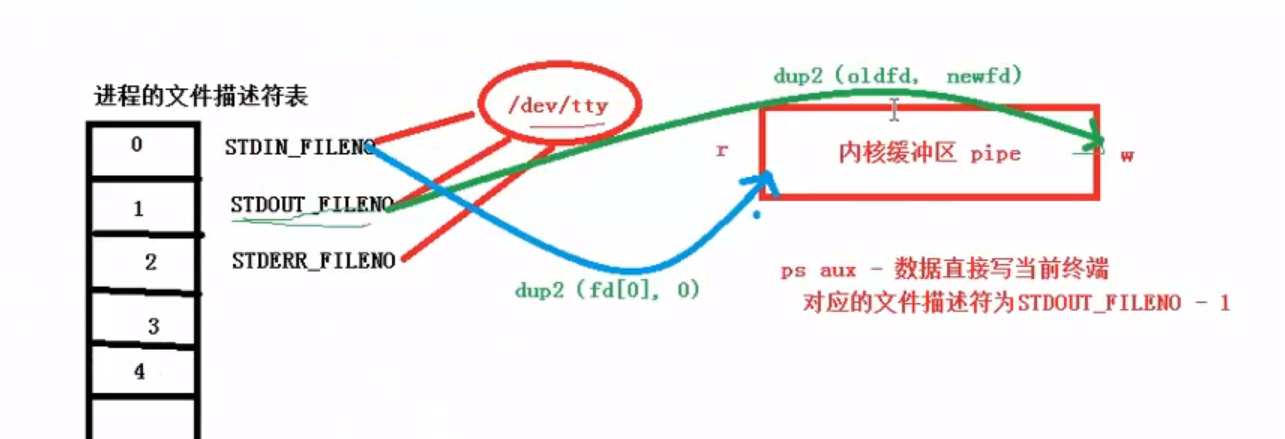
\includegraphics[scale=0.35]{psPipe.png}
				\caption{bash 管道原理分析图}
			\end{figure}
				
		\paragraph{fifo()}有名管道
			\subparagraph{函数原型}\fbox{int mkfifo(const char* path, mode\_t mode)}
			
			\subparagraph{说明}
				\begin{itemize}[itemindent = 1em]
					\item 内核缓冲区、有名管道
					\item 创建成功后磁盘会多一个文件,但是占用大小为0.
					\item 操作管道相当于操作文件
					\item 半双工、单向
					\item 没有血缘关系的进程间通信
					\item \verb|path |指定创建出来的伪文件名,用于间接指向管道缓冲区
					\item 读进程a打开\verb|path |指定的文件,读取
					\item 写进程b打开\verb|path |指定的文件,写
				\end{itemize}
				
	\section{内存映射}
		\paragraph{mmap()}创建内存映射,将文件映射到内存区,操作内存以替代操作文件,因此在操作时需要注意同步问题,因为内存不存在阻塞的属性。
			\subparagraph{函数原型}\fbox{void* mmap(void* addr, size\_t length, int prot, int flags, int fd, off\_t offset)}
		
			\subparagraph{说明}
				\begin{itemize}[itemindent = 1em]
					\item \textbf{返回值}
						\begin{enumerate}[itemindent = 1em]
							\item 成功 返回内存指针。
							\item 失败 返回\verb|MAP_FAILED|,等价于-1。
						\end{enumerate}
					\item \verb|*addr |映射区首地址,传\verb|NULL|
					\item \verb|lenght |映射区大小,4k 倍且不能为0,一般文件多大,length 就制定多大
					\item \verb|prot |映射区权限,\verb|PROT_READ 读权限 PROT_WRITE 写| 
					\item \verb|flags |标志位参数,
						\begin{enumerate}[itemindent = 1em]
							\item \verb|MAP_SHARED 共享 |表示修改了内存数据会同步到磁盘 
							\item \verb|MAP_PRIVATE 私有 |修改了内存不会同步到磁盘
						\end{enumerate}
					\item \verb|fd |文件描述符, 打开文件时权限必须大于等于prot
					\item \verb|offset |映射文件的偏移量,必须是4k(4096)的整数倍
				\end{itemize}
			
		\textbf{ 内存位置与原理}:\url{http://kdf5000.com/2017/02/17/mmap%E5%86%85%E5%AD%98%E6%98%A0%E5%B0%84/}
			\begin{figure}[H]
				\centering
				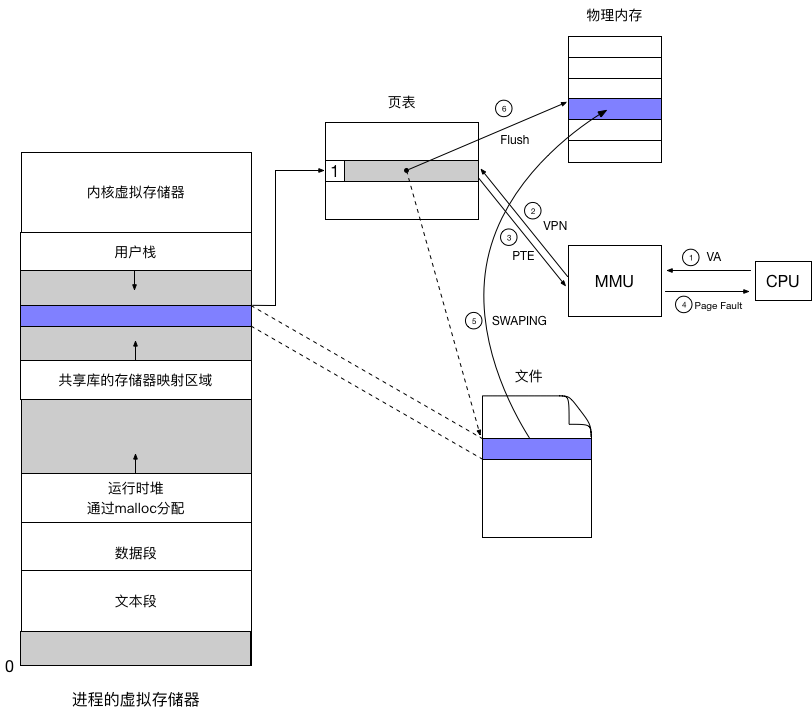
\includegraphics[scale=0.3]{mmap_pgfault.png}
				\caption{内存映射原理}
			\end{figure}		
			
			
		\paragraph{munmap()}释放内存映射区
			\subparagraph{函数原型}\fbox{int munmap(void* addr, size\_t length)}
		
			\subparagraph{说明}
				\begin{itemize}[itemindent = 1em]
					\item \verb|*addr |为\verb|mmap()|的返回值
					\item \verb|length |映射区大小
				\end{itemize}
		
		
		\paragraph{创建匿名内存映射}
			确定固定的参数,使得mmap()函数创建出匿名的内存映射,具体如下:
			
			\verb@void *ptr = mmap(NULL, len, PROT_READ|PROT_WRITE, MAP_SHARED | MAP_ANON, -1, 0)@
			
			主要修改内容有
				\begin{itemize}[itemindent = 1em]
					\item \verb|flags 权限| 添加宏\verb|MAP_ANON |说明是匿名内存映射
					\item \verb|fd |此处限定为-1,因为不存在文件了
					\item \verb|offset |此处限定为0, 因为不存在文件了
				\end{itemize}
		
		
		\paragraph{父子进程A、B如何使用内存映射通信}
			
			首先:\textbf{父子进程共享内存映射区}。因为共享映射区已经映射到内存中了,所以该处就是内存地址的复制。
						
		\paragraph{非血缘关系进程A、B如何使用内存映射通信}
			如何通信?
				\begin{itemize}[itemindent = 1em]
					\item \textbf{不能使用匿名映射}的方式
					\item \textbf{只能借助磁盘文件}创建映射区,假设文件为hello
					\item 内存映射区操作是\textbf{不阻塞}的
				\end{itemize}
				
				\subparagraph{实现}\verb|->|
				
					A 进程:
					\begin{lstlisting}[frame = L, xleftmargin = .1\textwidth]
	int fd = open("hello");
	void *ptr = mmap(,,,,fd,0);
	// 对映射区操作
	strcpy(ptr,"hello world!\n");
					\end{lstlisting}
					
					B 进程:
					\begin{lstlisting}[frame = L, xleftmargin = .1\textwidth]
	int fd2 = open("hello");
	void *ptr2 = mmap(,,,,fd2,0);
	// 对映射区操作
	cout<< *ptr2 <<endl;
					\end{lstlisting}
					
				\subparagraph{释放} 只有一个进程进行释放内存映射。
			
	\section{共享内存区}	
		\paragraph{shmget()}
	
	\section{信号}系统开销小
		\paragraph{产生、状态、处理方式}
			\subparagraph{产生}
				主要有5种方式,但是需要注意的是,信号是由内核产生发送的:
				\begin{itemize}[itemindent = 1em]
					\item \textbf{键盘}:\verb|ctrl+c| 等
					\item \textbf{命令}:\verb|kill|
					\item \textbf{系统函数}:\verb|kill()|
					\item \textbf{软条件}:定时器
					\item \textbf{硬件}:段错误、除0错误
				\end{itemize}
			\subparagraph{状态}
				主要分为三种方式:
				\begin{itemize}[itemindent = 1em]
					\item \verb|产生状态|
					\item \verb|未决状态|:信号未被处理
					\item \verb|递达状态|:信号被处理
				\end{itemize}
				
			\subparagraph{执行过程} 
				信号的优先级最高,当进程收到信号之后,暂停正在处理的工作,优先处理信号,处理完成之后再继续暂停的工作。	
		
			\subparagraph{处理方式}
				在信号的处理方式上,主要有以下5种方式:
				\begin{itemize}[itemindent = 1em]
					\item \verb|Term |终止进程
					\item \verb|Ign  |忽略信号
					\item \verb|Core |终止进程,并产生coreDump 文件用于调试
					\item \verb|Stop |暂停进程(挂起)
					\item \verb|Cont |恢复进程(恢复执行)
				\end{itemize}
			
			\subparagraph{信号帮助}
				\verb|man 7 signal|	
		
		\paragraph{kill()}发送信号给指定进程
			\subparagraph{函数原型}\fbox{int kill(pid\_t pid, int sig)}	
			
			\subparagraph{参数说明}
				\begin{itemize}[itemindent =1em]
					\item \verb|pid |指定的进程号  
					\item \verb|sig |指定的信号
				\end{itemize}
			
		\paragraph{raise()}自己给自己发信号
			\subparagraph{函数原型}\fbox{int raise(int sig)}	
			
			\subparagraph{参数说明}
				\begin{itemize}[itemindent =1em]
					\item \verb|sig |指定的信号
				\end{itemize}		
		
		\paragraph{abort()}给自己发送异常终止信号,永远不会调用失败
			\subparagraph{函数原型}\fbox{void abort()}	
		
		\paragraph{进程运行时间}\verb|->|
		
			\verb|time ./程序 |测试程序运行时间,计算如下。
		
			$$\verb|real = 用户 + 内核 + 损耗(文件I/O操作)| $$
				
		\paragraph{alarm()}设置定时器(每个进程只有一个定时器),使用的是自然定时法,不受进程状态影响
			\subparagraph{函数原型}\fbox{unsigned int alarm(unsigned int seconds)}	
			
			\subparagraph{参数说明}
				\begin{itemize}[itemindent =1em]
					\item 当时间到达后,函数发出一个信号\verb|SIGALRM|给自己的当前进程
					\item 只能相应一次
				\end{itemize}		
		
		\paragraph{setitimer()}
			\subparagraph{函数原型}\fbox{int setitimer(int which, const struct itimerval *new\_value, struct itimerval *old\_value)}	
			
			\subparagraph{参数说明}
				\begin{itemize}[itemindent =1em]
					\item \verb|struct itimerval|
						\begin{lstlisting}[frame = L, xleftmargin = .07\textwidth]
	struct itimerval{
		struct timeval it_interval; // 定时器循环周期
		struct timeval it_value; // 第一次触发定时器的时间
	};
						\end{lstlisting}
					\item \verb|struct timeval|
						\begin{lstlisting}[frame = L, xleftmargin = .07\textwidth]
	struct timeval{
		time_t tv_sec;	// 秒
		suseconds_t tv_usec; // 微秒
	};
						\end{lstlisting}
					\item \verb|which |:定时法则
						\begin{enumerate}[itemindent = 1em]
							\item \verb|ITIMER_REAL| = 用户 + 内核 + 损耗 
							\item \verb|ITIMER_VIRTUAL| = 用户
							\item \verb|ITIMER_PROF| = 用户 + 内核
						\end{enumerate}
				\end{itemize}				
	
		\paragraph{signal()}用于信号捕捉
			\subparagraph{函数原型}\fbox{sighandler\_t signal(int signum, sighandler\_t handler)}	
			
			\subparagraph{参数说明}
				\begin{itemize}[itemindent =1em]
					\item \verb|sighandler_t  = typedef void(*sighandler_t)(int);| 
					\item \verb|signum |要处理的信号
					\item \verb|handler | 处理函数的函数指针
				\end{itemize}	
	
		\paragraph{sigaction()}用于信号捕捉
			\subparagraph{函数原型}\fbox{int sigaction(int signum, const struct sigaction *act, struct sigaction *oldact)}	
			
			\subparagraph{参数说明}
				\begin{itemize}[itemindent =1em]
					\item \verb|signum |要处理的信号
					\item \verb|struct sigaction |
						\begin{lstlisting}[frame = L, xleftmargin = .07\textwidth]
	struct sigaction{
		void (*sa_handler)(int); // 处理函数
		void (*sa_sigaction)(int, siginfo_t*, void*);
		sigset_t sa_mask; // 信号集(内核区),在信号函数执行过程中,临时屏蔽指定的信号。函数执行完后,自动解除屏蔽
		int sa_flags; // 处理函数使用sa_handler 时赋值为0, 否则赋值为其他值
		void (*sa_restorer)(void);
	}
						\end{lstlisting}
					\item \verb|NULL|
				\end{itemize}	
		
		\paragraph{信号集相关}
			\subparagraph{未决信号集}
			
			\subparagraph{阻塞信号集}
			
			\subparagraph{sigemptyset()} 将set 集合置空
			
			\subparagraph{sigaddset()} 将信号加入集合
			
			\subparagraph{sigfillset()} 将所有信号加入set 集合
			
			\subparagraph{sigprocmask()} 屏蔽and接触信号屏蔽,将自定义信号集设置给阻塞信号集
			
			\subparagraph{sigpending()} 读取当前进程的未决信号集
	
			
	\section{socket}
		\paragraph{sock()}


\chapter{图形界面}
	\section{GTK-GNOME}
	
		
\chapter{库的使用}
	\url{http://www.cnblogs.com/52php/p/5681711.html}
	\section{介绍}
		使用GNU的工具我们如何在Linux下创建自己的程序函数库?一个“程序函数库”简单的说就是一个文件包含了一些编译好的代码和数据,这些编译好的代码和数据可以在事后供其他的程序使用。程序函数库可以使整个程序更加模块化,更容易重新编译,而且更方便升级。  
		
		引用的那些\textbf{头文件中的函数}是怎么被执行的呢?这就要牵扯到\textbf{链接库}了!
		
		库有两种,一种是 \textbf{静态链接库},一种是 \textbf{动态链接库},不管是哪一种库,\textit{要使用它们,都要在程序中包含相应的 include 头文件}。编译过程如下:
		
		\begin{figure}[H]
			\centering
			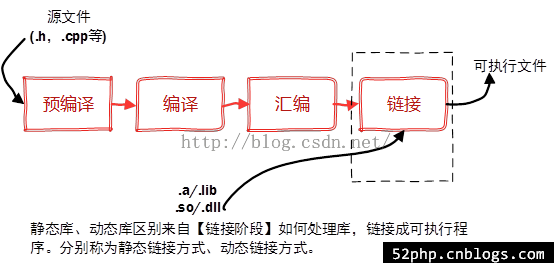
\includegraphics[scale = 0.7]{figure/compileProcess.png}
			\caption{编译过程}
		\end{figure}
		
		\verb|gcc -o helloWorld helloWorld.c| 生成一个helloWorld 的执行文件,格式为ELF(与widows的exe类似)。
		
	\section{静态函数库}是在程序执行前就加入到目标程序中去了;
	
		静态函数库实际上就是简单的一个普通的目标文件的集合,一般来说习惯用“\verb|.a|”作为文件的\textbf{后缀}
		
		静态库函数允许程序员把程序link起来而不用重新编译代码,节省了重新编译代码的时间。
		
		如你想把自己提供的函数给别人使用,但是又想对函数的源代码进行保密,你就可以给别人提供一个静态函数库文件。理论上说,使用ELF格式的静态库函数生成的代码可以比使用共享函数库(或者动态函数库)的程序\textbf{运行速度上快一些,大概1-5\%,但是占用空间却大了很多。}
			
			\subparagraph{Example}\verb|->|
				
				定义一个加法函数,做成静态库,首先需要将声明放到头文件以便引用。
				\begin{lstlisting}
	// add.h
	#ifndef _ADD_
	#define _ADD_
	#include <iostream>
	
	int add(int a, int b);
	#endif
				\end{lstlisting}
				
				实现该函数
				\begin{lstlisting}
	#include "add.h"
	
	int add(int a, int b)
	{
		return a+b;
	}
				\end{lstlisting}
			
				生成静态库:
				\begin{enumerate}[itemindent = 2em]
					\item \verb|g++ -c add.cc|生成\verb|.o|文件
					\item \verb|ar -crv libadd.a add.o|生成一个静态库
				\end{enumerate}
				
				
				测试:
				\begin{lstlisting}
	//目录结构
	project
		|
		+---Main.cc
		|
		+---addlib
				|
				+----add.h
				|
				+----add.cc
	
	#include <iostream>
	#include "./addlib/add.h"
	
	using namespace std;
	int main()
	{
		int num1 = 10;
		int num2 = 90;
		cout <<"the result is"<< add(num1,num2)<<endl;
		return 0;
	}
				\end{lstlisting}
				不管是哪一种库,\textit{要使用它们,都要在程序中包含相应的 include 头文件},所以include使用相对路径找到头文件\verb|add.h|
				
				然后我们使用\verb|g++ -o Test Main.cc -L ./addlib/ -ladd| 进行编译
				
				\begin{itemize}[itemindent = 2em]
					\item \verb|L |是指定加载库文件的路径
					\item \verb|l |是指定加载的库文件
				\end{itemize}
				
			\subparagraph{静态库搜索路径}\verb|->|
			
				\begin{enumerate}[itemindent= 2em]
					\item 编译目标代码时指定的静态库搜索路径。 \verb|-L ./src/ -lpthread|
					\item 环境变量\verb|LIBRARY_PATH| 指定的动态库搜索路径。
					
					 \verb|   export LIBRARY_PATH=/opt/lib:$LIBRARY_PATH|
					\item 配置文件\verb|/etc/ld.so.conf| 中指定的动态库搜索路径,然后运行\verb|/sbin/ldconfig|刷新缓存
					\item 默认的动态库搜索路径\verb|/lib, /usr/lib|
				\end{enumerate}
				
	\section{动态函数库}
		静态链接的话,文件会很大,往往实现很小的一个功能就需要占用很大的空间,而且每次库文件升级的话,都要重新编译源文件,很不方便。如下:
		\begin{figure}[H]
			\centering
			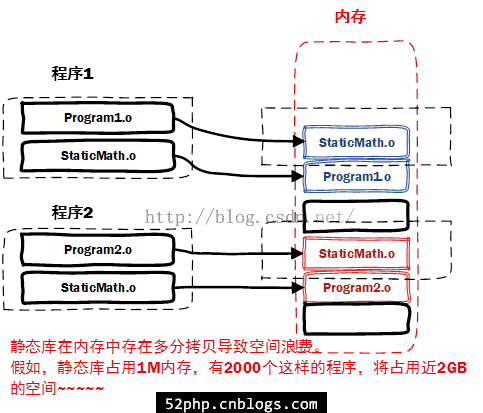
\includegraphics[scale = 0.7]{figure/staticLib-disAdvantage.png}
			\caption{静态库冗余空间}
		\end{figure}
		
		对于静态编译的程序1和程序2,都应用库staticMath。在内存中就又\textbf{两份相同的staticMath目标文件,很浪费空间},一旦程序数量过多就很可能会内存不足。
		
		这么大的内存才只能运行这几个程序,实在不甘心。
		这样就又了动态库发挥威力的地方了。我们来看看动态链接的结果:
		
		\begin{figure}[H]
			\centering
			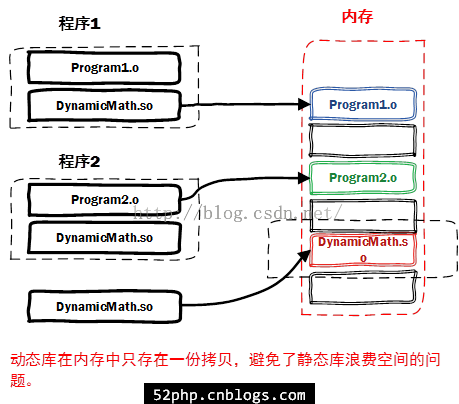
\includegraphics[scale = 0.7]{figure/dynamicLib.png}
			\caption{动态库解决静态库冗余空间问题}
		\end{figure}

		在这种模型中,两个程序只应用一个库,这个目标文件在内存中只有一份,供所有程序使用。
		并且在程序运行过程中动态调用库文件,\textbf{很方便,又不占空间},但是动态链接有一个\textbf{缺点就是可移植性太差},如果两台电脑运行环境不同,动态库存放的位置不一样,很可能导致程序运行失败。
			
		\subparagraph{Example}使用静态库代码结构与代码
		
		生成一个\verb|libadd.so|的动态库
		\verb|g++ -fPIC -shared -o libadd.so add.cpp|。
		这样就生成一个了一个libadd.so 的动态库。
		
		
		使用如下命令进行编译:
		\verb|g++ -o Test Main.cc -L ./addlib/ -ladd -Wl,-rpath=./addlib/|
		
		但是如果不指定运行时搜索路径的话,会出现cannot open shared obj错误。如下编译:
		
		\verb|g++ g++ -o Test Main.cc -L ./addlib/ -ladd|
		
		此时可以通过\verb|ldd ./Test|进行查看调用的动态库情况。具体的设置可参考动态库搜索路径的4种方法。
		
		
		\subparagraph{动态库搜索路径}\verb|->|
		
			\url{http://blog.csdn.net/weicao1990/article/details/51028335}			
			\url{https://www.cnblogs.com/cute/archive/2011/02/24/1963957.html}
			
			\begin{enumerate}[itemindent= 2em]
				\item 编译目标代码时指定的动态库搜索路径。\verb|-L./src/ -ladd -Wl,-rpath=./src/|
				
				\verb|   |前面两个\verb|-L -l|分别指明了动态库的位置和库的名字用于编译,只有引用, 后面的\verb|-Wl,-rpath|则指明运行时到哪里运行,有内容。
				
				\item 环境变量\verb|LD_LIBRARY_PATH| 指定的动态库搜索路径。
				
				\verb|   export LD_LIBRARY_PATH=/opt/lib:$LD_LIBRARY_PATH|
				\item 配置文件\verb|/etc/ld.so.conf| 中指定的动态库搜索路径,然后运行\verb|/sbin/ldconfig|刷新缓存
				\item 默认的动态库搜索路径\verb|/lib, /usr/lib|,\verb|mv ./src/xx.lib  /lib|
			\end{enumerate}

\chapter{工具}
	\section{gdb}
	
	
	\section{CMake}
	
				    
\end{document} 
 		    